\section{Discussion} \label{Sec: Discussion}
\subsection{Bolometric IR LF} \label{Sec: Bolometric IR LF}

\begin{itemize}
    \item \textcolor{red}{As previously discussed, the name of the python routines can be mentioned for experts or for people willing to reproduce the same results, but to the purpose of explaining what has been done in this work, they are totally irrelevant and do not substitute a detailed description of the fitting method and errors calculation. Please, provide information about the adopted techniques and their application to data.}
    \item \textcolor{Green}{Instead of saying the python terms and things, just say I use the least squares fitting or whatever.}
\end{itemize}

Figure \ref{Fig: Bolometric IR LF} presents the bolometric IR LFs derived from the ZFOURGE and CIGALE samples. This comparison allows us to explore the evolution of total IR emission and the individual contributions from SF and AGN across twelve redshift bins from $0 \leq z < 6$. By comparing the total LF from ZFOURGE with the decomposed SF and AGN LFs from CIGALE, we aim to better understand the distinct roles of SF and AGN activity in galaxy evolution over cosmic time. To model these LFs, we employ \texttt{scipy.optimize.curve\_fit} \citep{virtanen_scipy_2020} to perform the fitting and calculate 1$\sigma$ relative parameter dispersion errors using \texttt{np.sqrt(np.diag(pcov))} from \texttt{NumPy} \citep{harris_array_2020}. 

\subsubsection{ZFOURGE Total}
\begin{itemize}
    \item \textcolor{red}{Figure 3: what is shown in this figure is a very strange result, difficult to sell. }
    
    \item \textcolor{red}{It is hard to believe that the error bars at the faint end of the LFs are so small, especially given the fact that the total IR Luminosity for these faint objects has likely been obtained without benefitting of far-IR data. Please, discuss the data used for the SED-fitting and perform a detailed uncertainty analysis through opportune simulations.}
    
    \item \textcolor{red}{I do not understand how it is possible that the total LF is much lower than the SF component one around the knee in most redshift bins up to z=3. I would expect it to be consistent with the sum of the two, AGN+SF: why this happens? Please, justify this odd result.}
    
    \item \textcolor{red}{Moreover, how can be explained that the bright end of the total ZFOURGE LF at z>3 is so Much higher than the AGN LF one? I would have expected the AGN to make most of the bright-end.}
    
    \item \textcolor{red}{Also, the explanation about the inconsistency with literature results in the z=1.7-2 bin is difficult to be the correct one: incompleteness should have affected the higher redshift bin, not the one where both Rodighiero+10 and Gruppioni+13 samples contained the bulk of objects, then followed by a bin where no apparent drop in number is observed.}
    \item \textcolor{Green}{I need to look at this}
    
    \item \textcolor{red}{All the discussion in Section 5.1.2, 5.1.3 and 5.1.4 has no meaning if one cannot believe in the results shown in Figure 3.}
    
    \item \textcolor{red}{I stress again, once resolved the inconsistency issue in the LFs normalisation, the authors should adopt the same form to fit the data LFs of the different components. Otherwise, the comparison is meaningless}
    \textcolor{Green}{ANother one of these. Motivation si to compare to the literature. Schechter to SF and Saunders to AGN. They are not necessarily a direct comparison. Reiterate this is not a comparison of decomposed vs fourge. Its a comparion between better luminosity estimates. ZFOURGE would have had this luminsotiy function before decomposition exists. Now we have a better way of measuring luminosity.}
\end{itemize}

Focusing first on the ZFOURGE data, we compare our results with \cite{rodighiero_mid-_2010} and \cite{gruppioni_herschel_2013}. We also compare our results with \cite{huang_local_2007, caputi_infrared_2007, fu_decomposing_2010} but avoid cluttering figure \ref{Fig: Bolometric IR LF} with these disjointed redshift bins from the literature. Across all redshift bins (except the most local), we consistently see that the ZFOURGE number density ($\phi$) values in blue extend much fainter than the rest of the literature, showcasing ZFOURGE's ability to probe to fainter luminosities. However, there remains room to improve the constraints at the faint end of the ZFOURGE LF. Extending the analysis by an additional order of magnitude fainter in each redshift bin would significantly enhance our ability to constrain the faint-end slope.

\begin{figure}
    \centering
    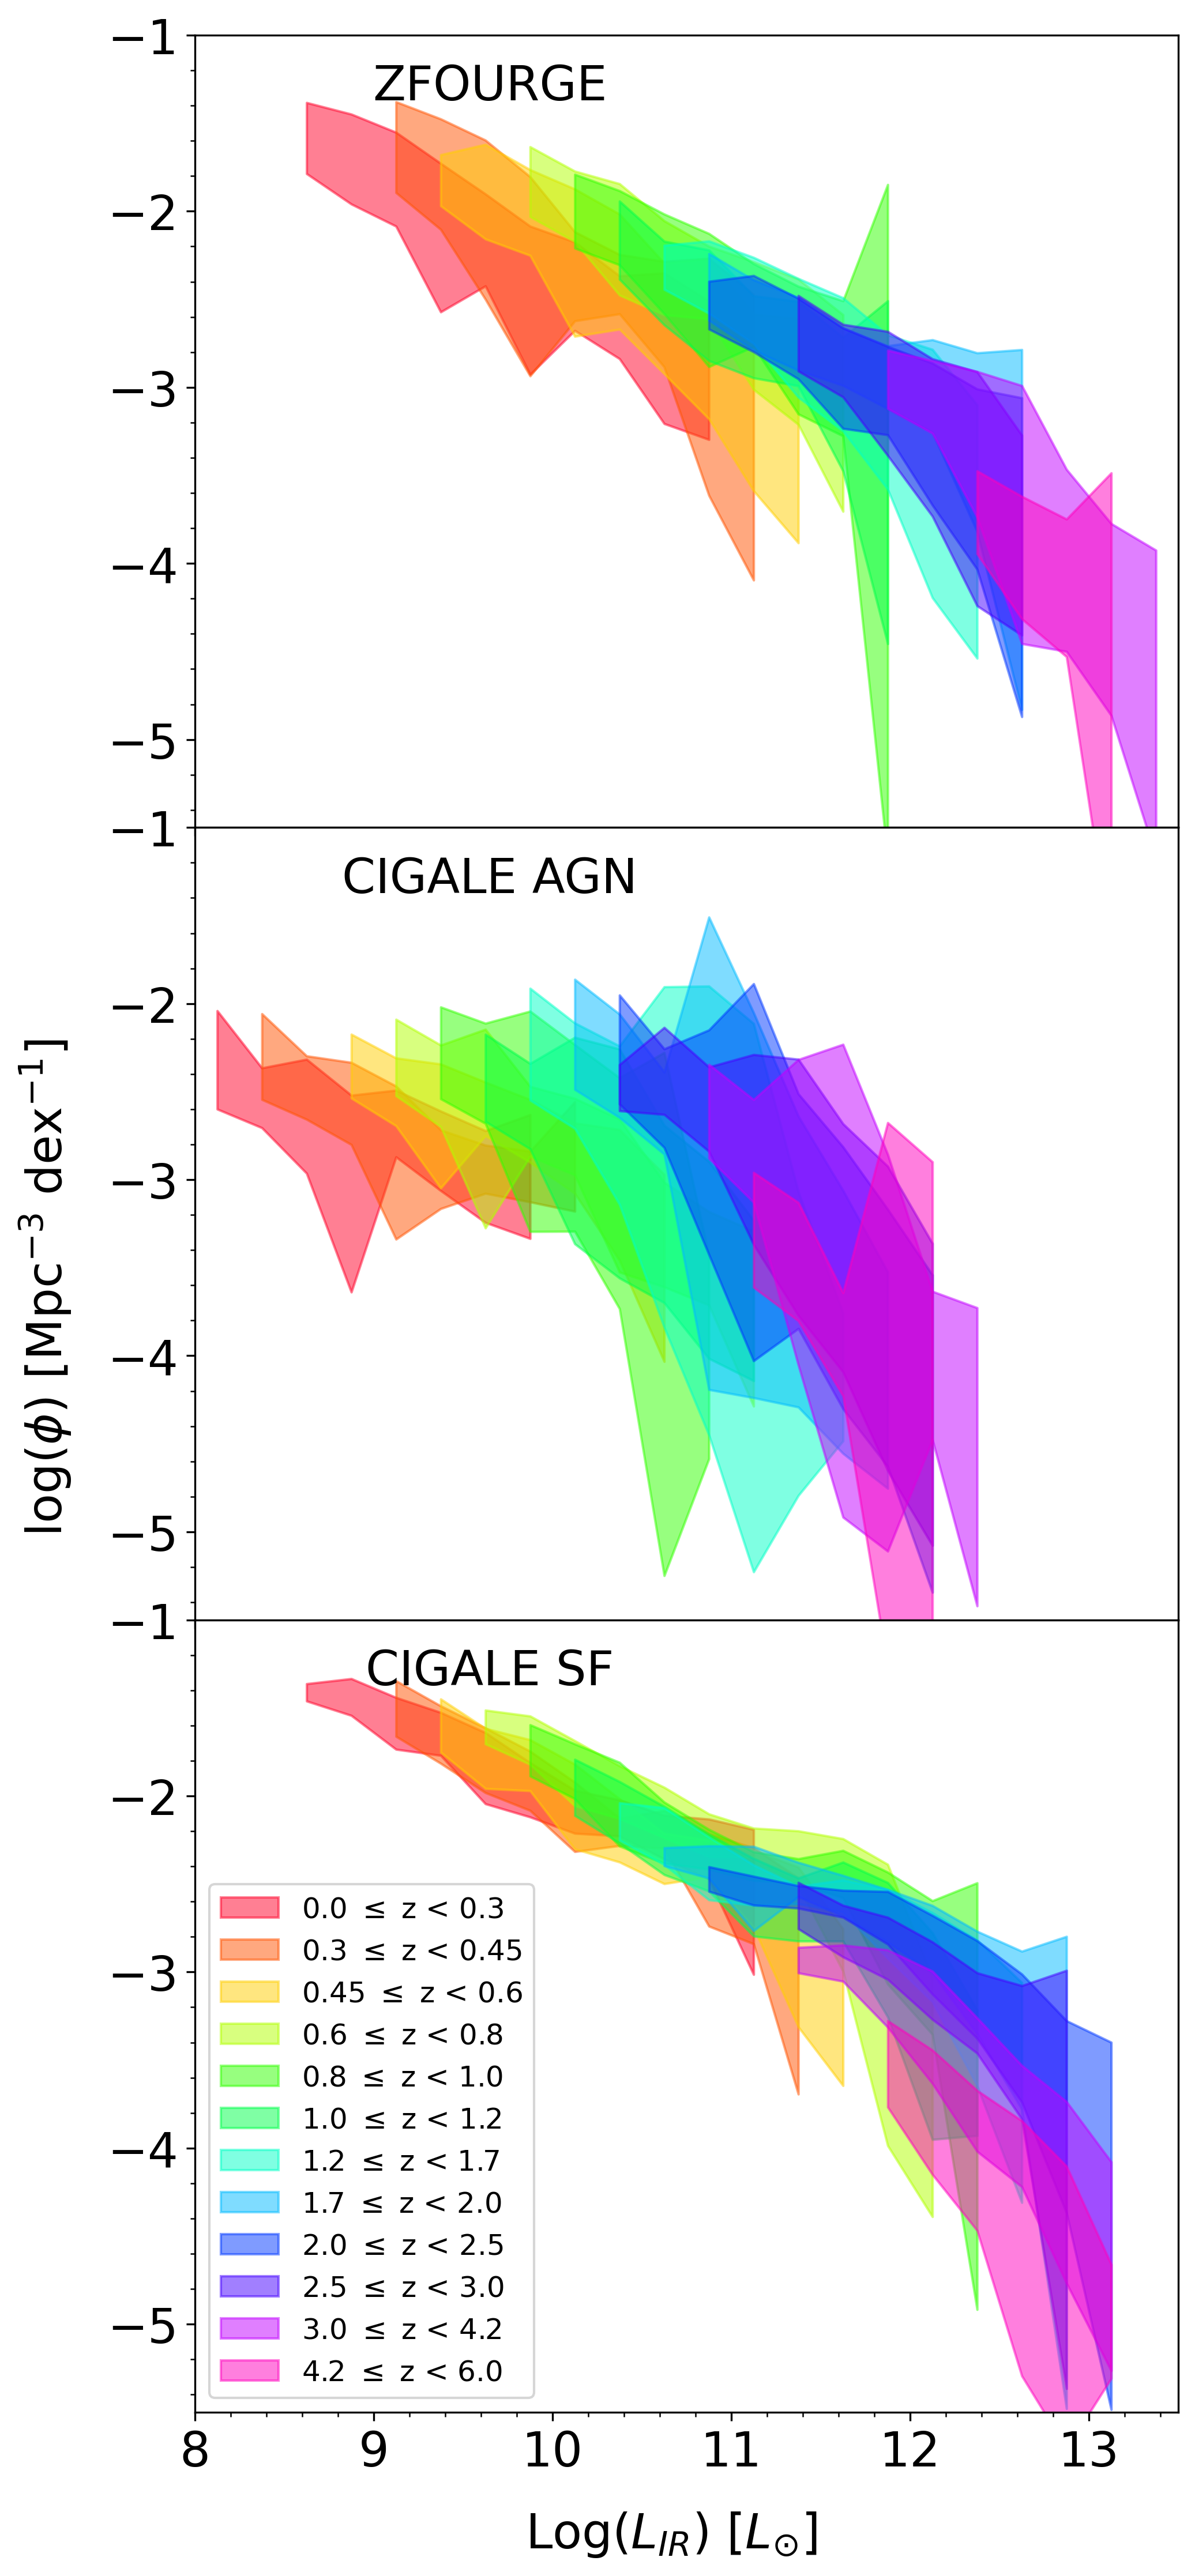
\includegraphics[width=0.48\textwidth]{Figures/LF_Filled.png}
    \caption{Combined evolution of the ZFOURGE total (top), CIGALE AGN (middle), and CIGALE SF (bottom) luminosity functions shown in figure \ref{Fig: Bolometric IR LF}. The redshift evolution of each binned LF is easier to visualise. Data points are shaded between the $1\sigma$ uncertainties and coloured by redshift bin.}
    \label{Fig: LF Filled}
\end{figure}

Our ZFOURGE results agree very well with the literature in all bins except $1.7 \leq z < 2$ and $3.0 \leq z < 4.2$. In these redshift bins, ZFOURGE results show $\phi$ values $\approx 0.5$ dex higher across all luminosity bins when compared to the literature \citep{rodighiero_mid-_2010, gruppioni_herschel_2013}. We posit that ZFOURGE is detecting fainter sources in these redshift bins than previously observed. From $1.7 \leq z < 2$, both \cite{rodighiero_mid-_2010} and \cite{gruppioni_herschel_2013} show a drop in their faintest luminosity bins, consistent with incompleteness. \cite{gruppioni_herschel_2013} sees a decline of $\approx$ 0.5 log($\phi$) or more in each luminosity bin from $3.0 \leq z < 4.2$ when compared to their previous redshift bin and is likely to be solely an incompleteness issue given it is their final redshift bin. The fact that both \cite{gruppioni_herschel_2013} and \cite{rodighiero_mid-_2010} see a drop from $1.7 \leq z < 2$ is intriguing. This issue does not appear in neighbouring redshift bins or other redshift bins. \cite{rodighiero_mid-_2010} utilises multiwavelength Spitzer observations, whereas \cite{gruppioni_herschel_2013} uses Herschel/PACS data to estimate the total IR LF. Given that this incompleteness exists across multiple surveys and instruments, it remains to be seen why a drop in the $1.7 \leq z < 2$ redshift bin exists when neighbouring redshift bins show no sign of incompleteness. Similar can be said about our final redshift bin $4.2 \leq z < 6.0$ (figure \ref{Fig: Bolometric IR LF}). Luminosity bins in this redshift range show a drop along the faint end slop of our LF. Therefore, the redshift bin $4.2 \leq z < 6.0$ is likely incomplete and should be taken as a lower limit.

\subsubsection{CIGALE AGN}
For the CIGALE AGN, we compare our results with \cite{delvecchio_tracing_2014, symeonidis_agn_2021} and \cite{thorne_deep_2022}. \cite{symeonidis_agn_2021} derives their IR AGN $\phi$ values from the hard X-ray LFs by \cite{aird_evolution_2015}. \cite{thorne_deep_2022}, who performs similar work to this analysis, uses the SED fitting code \texttt{ProSpect} \citep{leja_deriving_2017, robotham_prospect_2020} to decompose the bolometric IR LF and recover the pure AGN component to the LF. We fit the Saunders function in red and $1\sigma$ uncertainties to our CIGALE decomposed AGN LF. We include \cite{thorne_deep_2022} AGN in our fitting process as we do not have comparatively bright AGN to constrain the bright end of the LF. 

In the first few redshift bins from $0 \leq z < 0.8$, our CIGALE AGN LF and the Saunders function fits are generally consistent with the results in the literature. However, the literature LFs tend to flatten considerably at higher redshifts and fainter luminosities. In contrast, our CIGALE AGN LFs do not flatten and instead continue to rise, suggesting that CIGALE SED decomposition is effective in isolating and recovering the AGN contribution to luminosities as faint as $10^8$ $L_{\odot}$. Furthermore, we probe fainter than \cite{thorne_deep_2022} whose faintest luminosity bins are never less than $10^{10}$ $L_{\odot}$ when accounting for completeness limits. While our CIGALE AGN lacks $\phi$ values at the brighter end of the LF, necessitating the use of \cite{thorne_deep_2022} $\phi$ values to constrain our Saunders function fits, CIGALE's ability to extend the LF to such faint luminosities provides crucial insights into the AGN population at higher redshifts.

Because the IR AGN identified by \cite{symeonidis_agn_2021} are derived from the hard X-ray LF presented by \cite{aird_evolution_2015}, the observed flattening at fainter luminosities is almost certainly due to X-ray emission not identifying the obscured faint AGN population. In contrast, SED fitting, as applied in our study, allows us to recover these faint AGN, providing a more complete picture of the AGN population \citep{gruppioni_modelling_2011, brown_infrared_2019, thorne_deep_2022}. Although not shown in Figure \ref{Fig: Bolometric IR LF}, the combined type-1 and type-2 AGN from \cite{symeonidis_agn_2021} show elevated number densities, particularly in the $1.2 \leq z < 2.5$ range, and align well with our CIGALE AGN results. This strong agreement underscores the robustness of our approach in isolating obscured faint AGN, especially at higher redshifts.

As the CIGALE AGN LF evolves with redshift, the faint end approaches the number density values of the CIGALE SF LF (discussed in the following subsection) at $0 \leq z < 2.5$ and nearly surpasses them at $z > 2.5$. This trend aligns with the well-known peak of the cosmic SF of galaxies above $z=2$ \citep{madau_cosmic_2014}. Conversely, the AGN fraction increases with redshift and $L_{IR}$ as noted by \cite{symeonidis_agn_2021, thorne_deep_2022} and references therein. Although our results do not yet show AGN number densities overtaking those of SF galaxies, future studies probing higher redshifts will likely reveal this transition, reflecting the dominance of AGN activity in the extremely early universe.

\subsubsection{CIGALE SF}
As seen in figure \ref{Fig: Bolometric IR LF}, the CIGALE SF LF is elevated above the ZFOURGE total and comparable literature LFs at brighter luminosities. We see excellent agreement between CIGALE SF and ZFOURGE LFs towards fainter luminosities. Several factors could contribute to this result. Work by \cite{wu_mid-infrared_2011} has shown that the UV and optical wavelengths follow a Schechter function closely. In contrast, the IR wavelengths have a shallower exponential which is inconsistent with a Schechter function \citep{symeonidis_what_2019}. \cite{fu_decomposing_2010} proposed that this difference is due to the AGN contribution to the IR Galaxy LF. \cite{wu_mid-infrared_2011} also concludes that the bright end slope is consistent with a Schechter function when AGN are removed. Given these findings, we argue that CIGALE accurately isolates the SF fraction and AGN contribution to galaxy emission. Although our results in figure \ref{Fig: Bolometric IR LF} show fewer luminosity bins at the bright end, there are enough to constrain a well-defined Schechter functional fit.

As expected, the bright-end slope of a Schechter function is too steep to accurately describe the ZFOURGE total IR LF \citep{wu_mid-infrared_2011}, in agreement with the literature \citep{rodighiero_mid-_2010, gruppioni_herschel_2013, symeonidis_what_2019}. Even after removing AGN-identified galaxies (552, \citealp{cowley_zfourge_2016}), the ZFOURGE LFs do not show an improved Schechter function fit as predicted by \cite{fu_decomposing_2010, wu_mid-infrared_2011}. The most likely reason is that \cite{cowley_zfourge_2016} only identifies the most AGN-dominated sources, leaving fainter-luminosity AGN undetected. AGN activity and SFR are tightly coupled (\citealp{alexander_what_2012} and references within), with both AGN activity and SF likely happening at the same time or in offset cycles \citep{cowley_decoupled_2018}. At higher redshifts ($z > 2$), it becomes increasingly essential to disentangle AGN and SF components of galaxy emission to model galaxy evolution accurately.

\subsubsection{Combined Evolution}
In figure \ref{Fig: LF Filled}, we show the combined evolution of the ZFOURGE bolometric IR (8-1000$\mu$m) LF. The LF is filled between the $1\sigma$ uncertainty bounds, calculated using equation \ref{EQ: Vmax Error}. With this figure, it is easier to see the evolution of the LF across luminosity and redshift. A clear declining density trend is seen with increasing luminosity and redshift.

This result is significant because it highlights how the relative contributions of SF and AGN activity evolve. Both SF and AGN number densities increase with luminosity as the universe ages towards the present day. This suggests a tentative downsizing effect, which we explore further in section \ref{Sec: Class Density}. The decline in the LF with increasing luminosity and redshift suggests that the early universe contained fewer luminous galaxies, implying lower overall SF and AGN activity. As we move towards the present day, the rising number density of bright galaxies in the LF (until the lowest redshift bins) reflects the growth and evolution of galaxies and their central SMBHs, with an increase in both SF and AGN contributions.

% \begin{itemize}
%     \item \textcolor{red}{is CIGALE AGN to be believed?}
%     \item \textcolor{red}{CIAGLE SF above ZFOURGE total}
%     \item \textcolor{red}{CIGALE/ZFOURGE lack bright end data}
% \end{itemize}

% The ZFOURGE quiescent LF is shown in figure \ref{Fig: Bolometric IR LF}. Quiescent luminosity bins are present in all but the highest redshift bin, after which the remaining quiescent galaxies fall below our minimum number count of 5 galaxies. The quiescent and SF galaxies follow an 80\% completeness limit that is very similar to the ZFOURGE total limit.

% We use AGN selection catalogues provided by \cite{cowley_zfourge_2016} to remove AGN identified sources from the galaxy, SF, and quiescent luminosity functions. 

% The completeness limit for each redshift bin was defined in section \ref{sec: Bolometric IR Luminosity}, are listed in table \ref{tab:bolo flux limits}, and shown as violet dashed lines in figure \ref{Fig: Bolometric IR LF}. Galaxies whose maximum comoving-distance is located at the end of the redshift bin, but have luminosities below the luminosity-distance limit are removed. The only galaxies in each redshift bin are galaxies whose maximum distance is the end of the redshift bin and thus galaxies whose maximum distance is less than the end of the redshift bin are removed.

% CIGALE could be overestimating the SF component of IR SEDs, overestimating the total IR energy density, or underestimating other components like the AGN contribution. It could also be that ZFOURGE's bolometric IR luminosity was underestimated. 

% The reader might now be wondering: is \texttt{CIGALE} to be believed? 

% The local \cite{sanders_iras_2003} luminosity function is shown across all redshift bins as the grey dashed line. 

% \textcolor{red}{Again, we remind the reader that our redshift bin $4.2 \leq z < 6.0$ is likely incomplete and should be taken as a lower limit. Nevertheless, the downwards evolutionary trend is still observed.}

% across redshift bins from $0\leq z < 2.5$ as gold stars and

% as purple crosses from $0\leq z < 4.2$

% from $0 \leq z < 2.5$ as pink hexagons and

% from $0 \leq z < \approx 2$